\documentclass[11pt]{article}
\usepackage{../cs70,latexsym,epsf}
\lecture{21}
\def\title{Lecture \the\lecturenumber}

\def\Ex#1{{\rm E}(#1)}
\def\Var#1{{\rm Var}(#1)}

\newcounter{thm}
\addtocounter{thm}{\the\lecturenumber}
\newtheorem{corollary}{Corollary}[thm]
\newtheorem{theorem}{Theorem}[thm]
\newtheorem{definition}{Definition}[thm]
\newtheorem{remark}{Remark}[thm]

\def\X{\mathcal{X}}
\def\Y{\mathcal{Y}}

\begin{document}

\maketitle

\section*{Inference}

In this note we revisit the problem of {\em inference}: 
Given some data or observations from the world, what can we infer about the underlying process that generates the data? The primary tool that allows us to make such an inference is {\em Bayes' rule}. We have seen some simple examples of Bayesian inference in Note~14, all of which can be modeled using the balls and bins model. In this note, we will build on this simple model to solve a machine learning application, namely the task of digit classification.


%%%%%%%%%%%%%%
\subsection*{Digit Classification}

Handwriting recognition is an important machine learning problem that has many practical applications. Many institutions nowadays regularly use automated systems to recognize handwriting and convert it to digital words or letters, which are easier to process and more efficient than having a human manually look at them one by one. For example, the post office uses handwriting recognition to detect the addresses on mail and sort them to the corresponding destinations, while banks use handwriting recognition to detect the amount of money that are written on checks. These systems have been fine-tuned and achieve accuracy comparable to (or even better than) human performance, which is why they are now so widely used.

To understand how these kinds of systems work, let us consider a simpler problem of digit classification. In this problem, we are given an image of a handwritten digit ($0-9$) and we have to identify the number written on the image. This is an instance of a {\em classification} problem: we are given an object (in this case an image) that belongs to one of several classes (the digits), and we have to decide which class to assign the object to. A typical dataset that is used for this problem is the MNIST\footnote{\url{http://yann.lecun.com/exdb/mnist/}} dataset, where each image is grayscale and has size $28 \times 28$ pixels. Figure~\ref{fig:digits} shows some examples of the digits from MNIST.

\begin{figure}[h!]
\centering
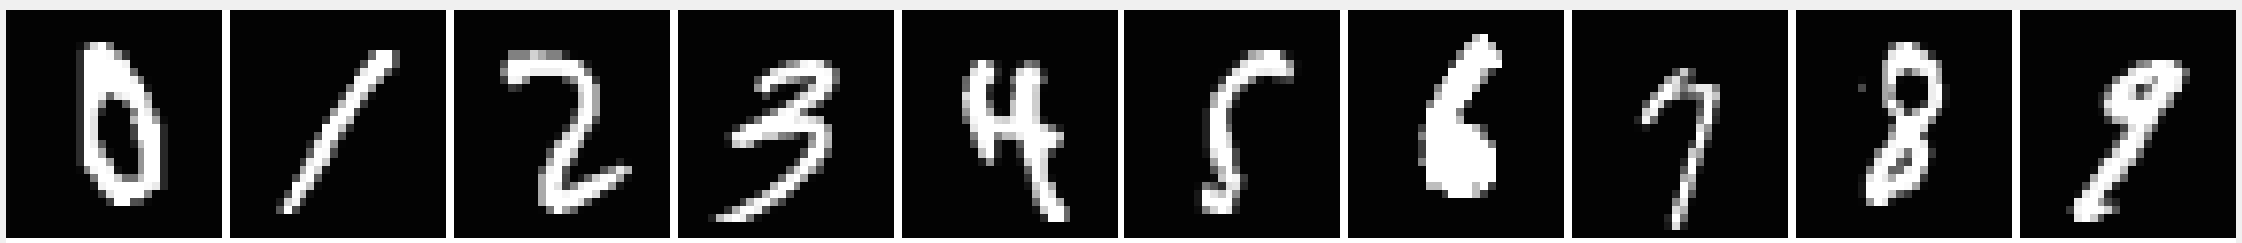
\includegraphics[scale=0.35]{digits.png}
\caption{Some examples of handwritten digit images from the MNIST dataset.}
\label{fig:digits}
\end{figure}

When we look at the images above, it seems easy for us (humans) to identify the digits. For example, the first image above is clearly a ``0'' because it looks like a circle, and we know it has to be a ``0''; similarly, the second image above is a ``1'' because it looks like a ``1'' from our experience, and so on. But in doing so, we are utilizing all our human knowledge and experience with digits. So it is our very good internal understanding of what constitutes a digit that is helping us recognize the digits easily. But if you were a computer, how would you go about approaching this problem?


%%%%%%%%%%%%%%%%%%%%%%%
\subsection*{Building a model of the digits}

We can imagine that if we have a good understanding of how the digits are generated, then we can solve the digit classification problem easily. For example, suppose for each digit $j$ you have a model $M(j)$ that can generate all possible images corresponding to that digit. Then given an image $x$, we can identify what digit is written in the image by checking which of the models $M(0),\dots,M(9)$ can generate $x$. If we have a perfect model for the digits, then there should be only one model $M(j)$ that can possibly generate the image $x$; all other models should reject $x$ as being inconsistent with their digit models. In this case, classification is easy: Given an image $x$, find the unique model $M(j)$ consistent with $x$, and classify $x$ as having digit $j$.

Following the argument above, we can try to find a good model for each digit. A reasonable first attempt is to come up with a list of simple rules for writing digits. For example, we can say that ``0'' looks like a circle, ``1'' looks like a vertical stroke, ``8'' looks like two stacked circles, and so on. But we immediately see that these simple rules are not sufficient to capture the wide variations among handwritten digits; see Figure~\ref{fig:digits2} for some more examples from the MNIST dataset.

\begin{figure}[h!]
\centering
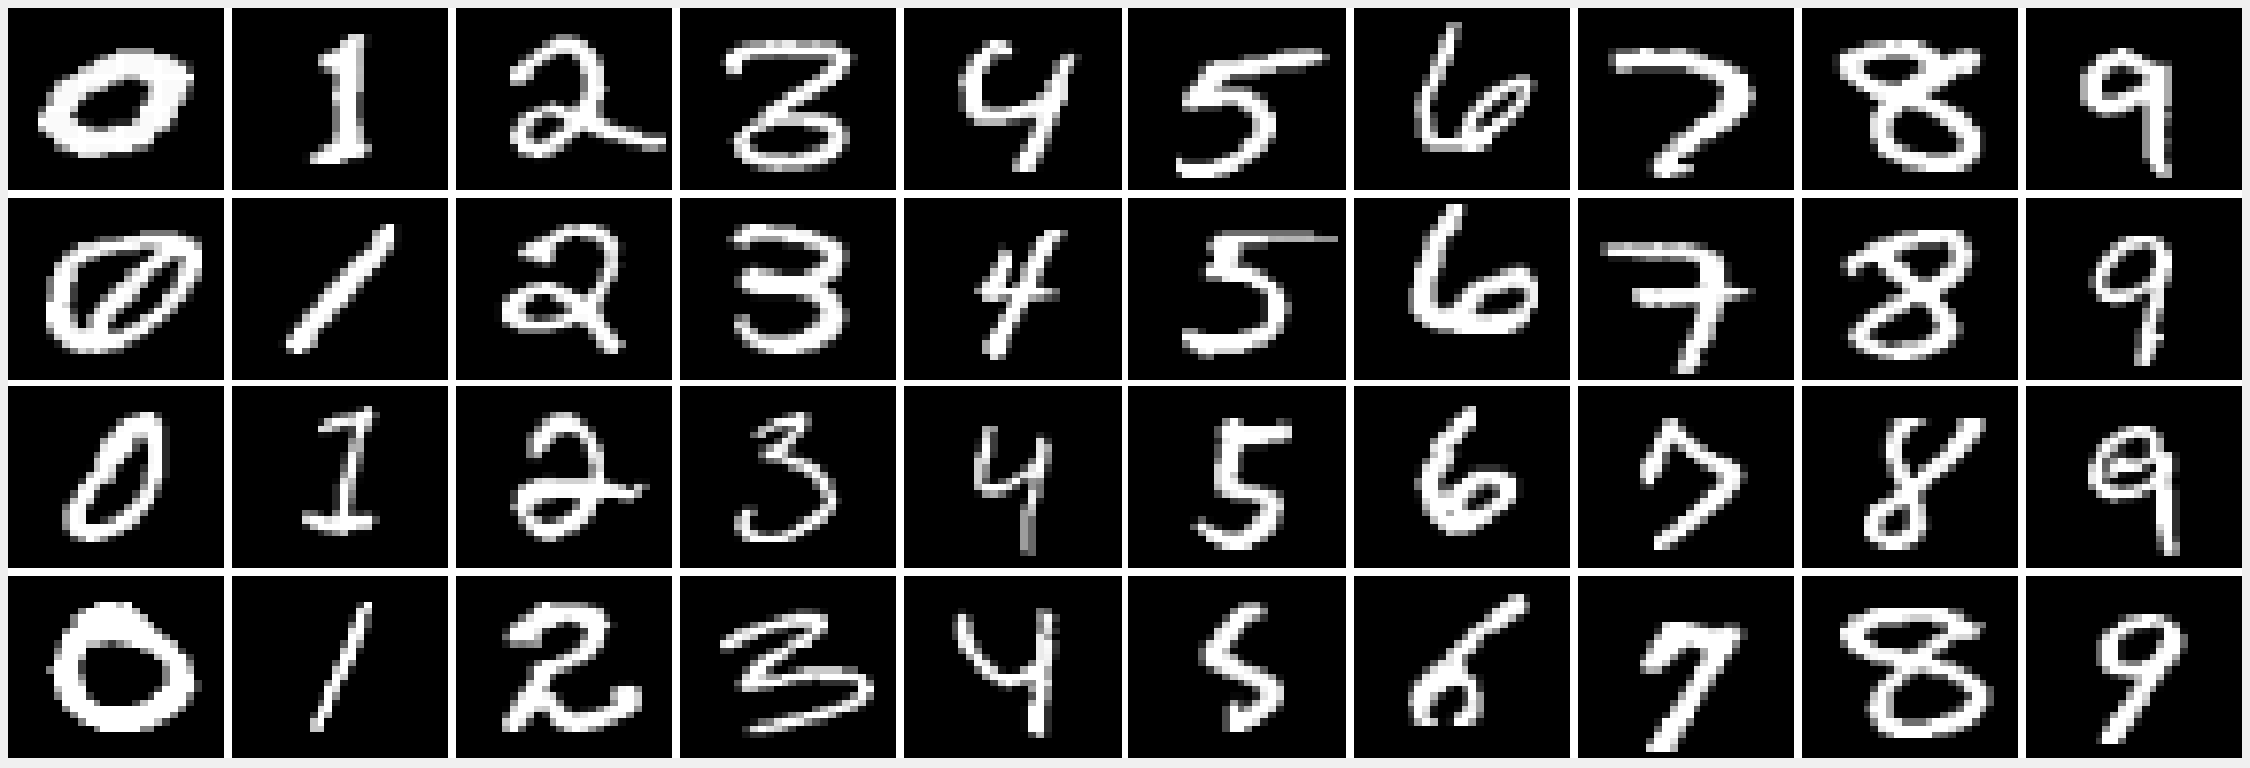
\includegraphics[scale=0.35]{digits2.png}
\caption{More examples of digit images from the MNIST dataset.}
\label{fig:digits2}
\end{figure}

Notice that some of the digits above do not follow standard simple rules that we may have come up with. For example, the second image of ``0'' has an additional stroke inside, yet we can still recognize it as a ``0''; similarly, the last image of ``5'' is missing the top horizontal stroke, but we know it is still a ``5''. If we want to be able to recognize these cases, we need to augment our list of rules to take into account all the possible ways to write digits. But even if the same person writes the same digit multiple times, we still see some variations in the result. So this rule-based approach will give us a very large set of rules that becomes unwieldy to use, and we can never be sure that we have captured all the possible variations.

We can try to come up with better models for digits that are more accurate. For example, we can consider modeling the curvature of the digits (how the angles between adjacent points in the digit change), or even start modeling the physical process of writing itself. But trying to capture the underlying variations in a realistic way requires a lot of sophistication, and at some point that task becomes more difficult than the original problem of digit classification that we started with.

So can we get away with a simpler model? The answer is yes: We can indeed use very simple, crude models for the digits. These simple models are themselves not too realistic, but in conjunction with Bayes' rule and the formalism of inference, we can still use them to get a good performance on our digit classification problem.




%%%%%%%%%%%%%%%%%%%%%%%
\subsection*{Probabilistic approach}

Recall that the difficulty in the problem is that we don't have a good concise definition that separates one digit from another. Indeed, there are many variations in writing a digit, as we saw in Figure~\ref{fig:digits2}. Our approach now is to take a {\em probabilistic view} of the problem: We treat the variations in the digits as a probability distribution over the images. So for each digit $j \in \{0,1,\dots,9\}$, we have a probability distribution $P_j(x)$ over the images $x$, which represents our uncertainty or imperfect knowledge about the variations among the images containing digit $j$.

Under distribution $P_j(x)$, we are a lot more likely to generate images $x$ that look like how we would write digit $j$; however, there is also a small probability that $P_j(x)$ generates images that are supposed to contain digit $j$, but by random chance may look like other digits. Figure~\ref{fig:P1x} shows an illustration of the distribution $P_1(x)$. The bulk of the mass (images that are assigned high probability) are good images of digit $1$, while on the tails (images with small probability) are some ambiguous images that could be interpreted as digit $1$, or possibly other digits.

\begin{figure}[h!]
\centering
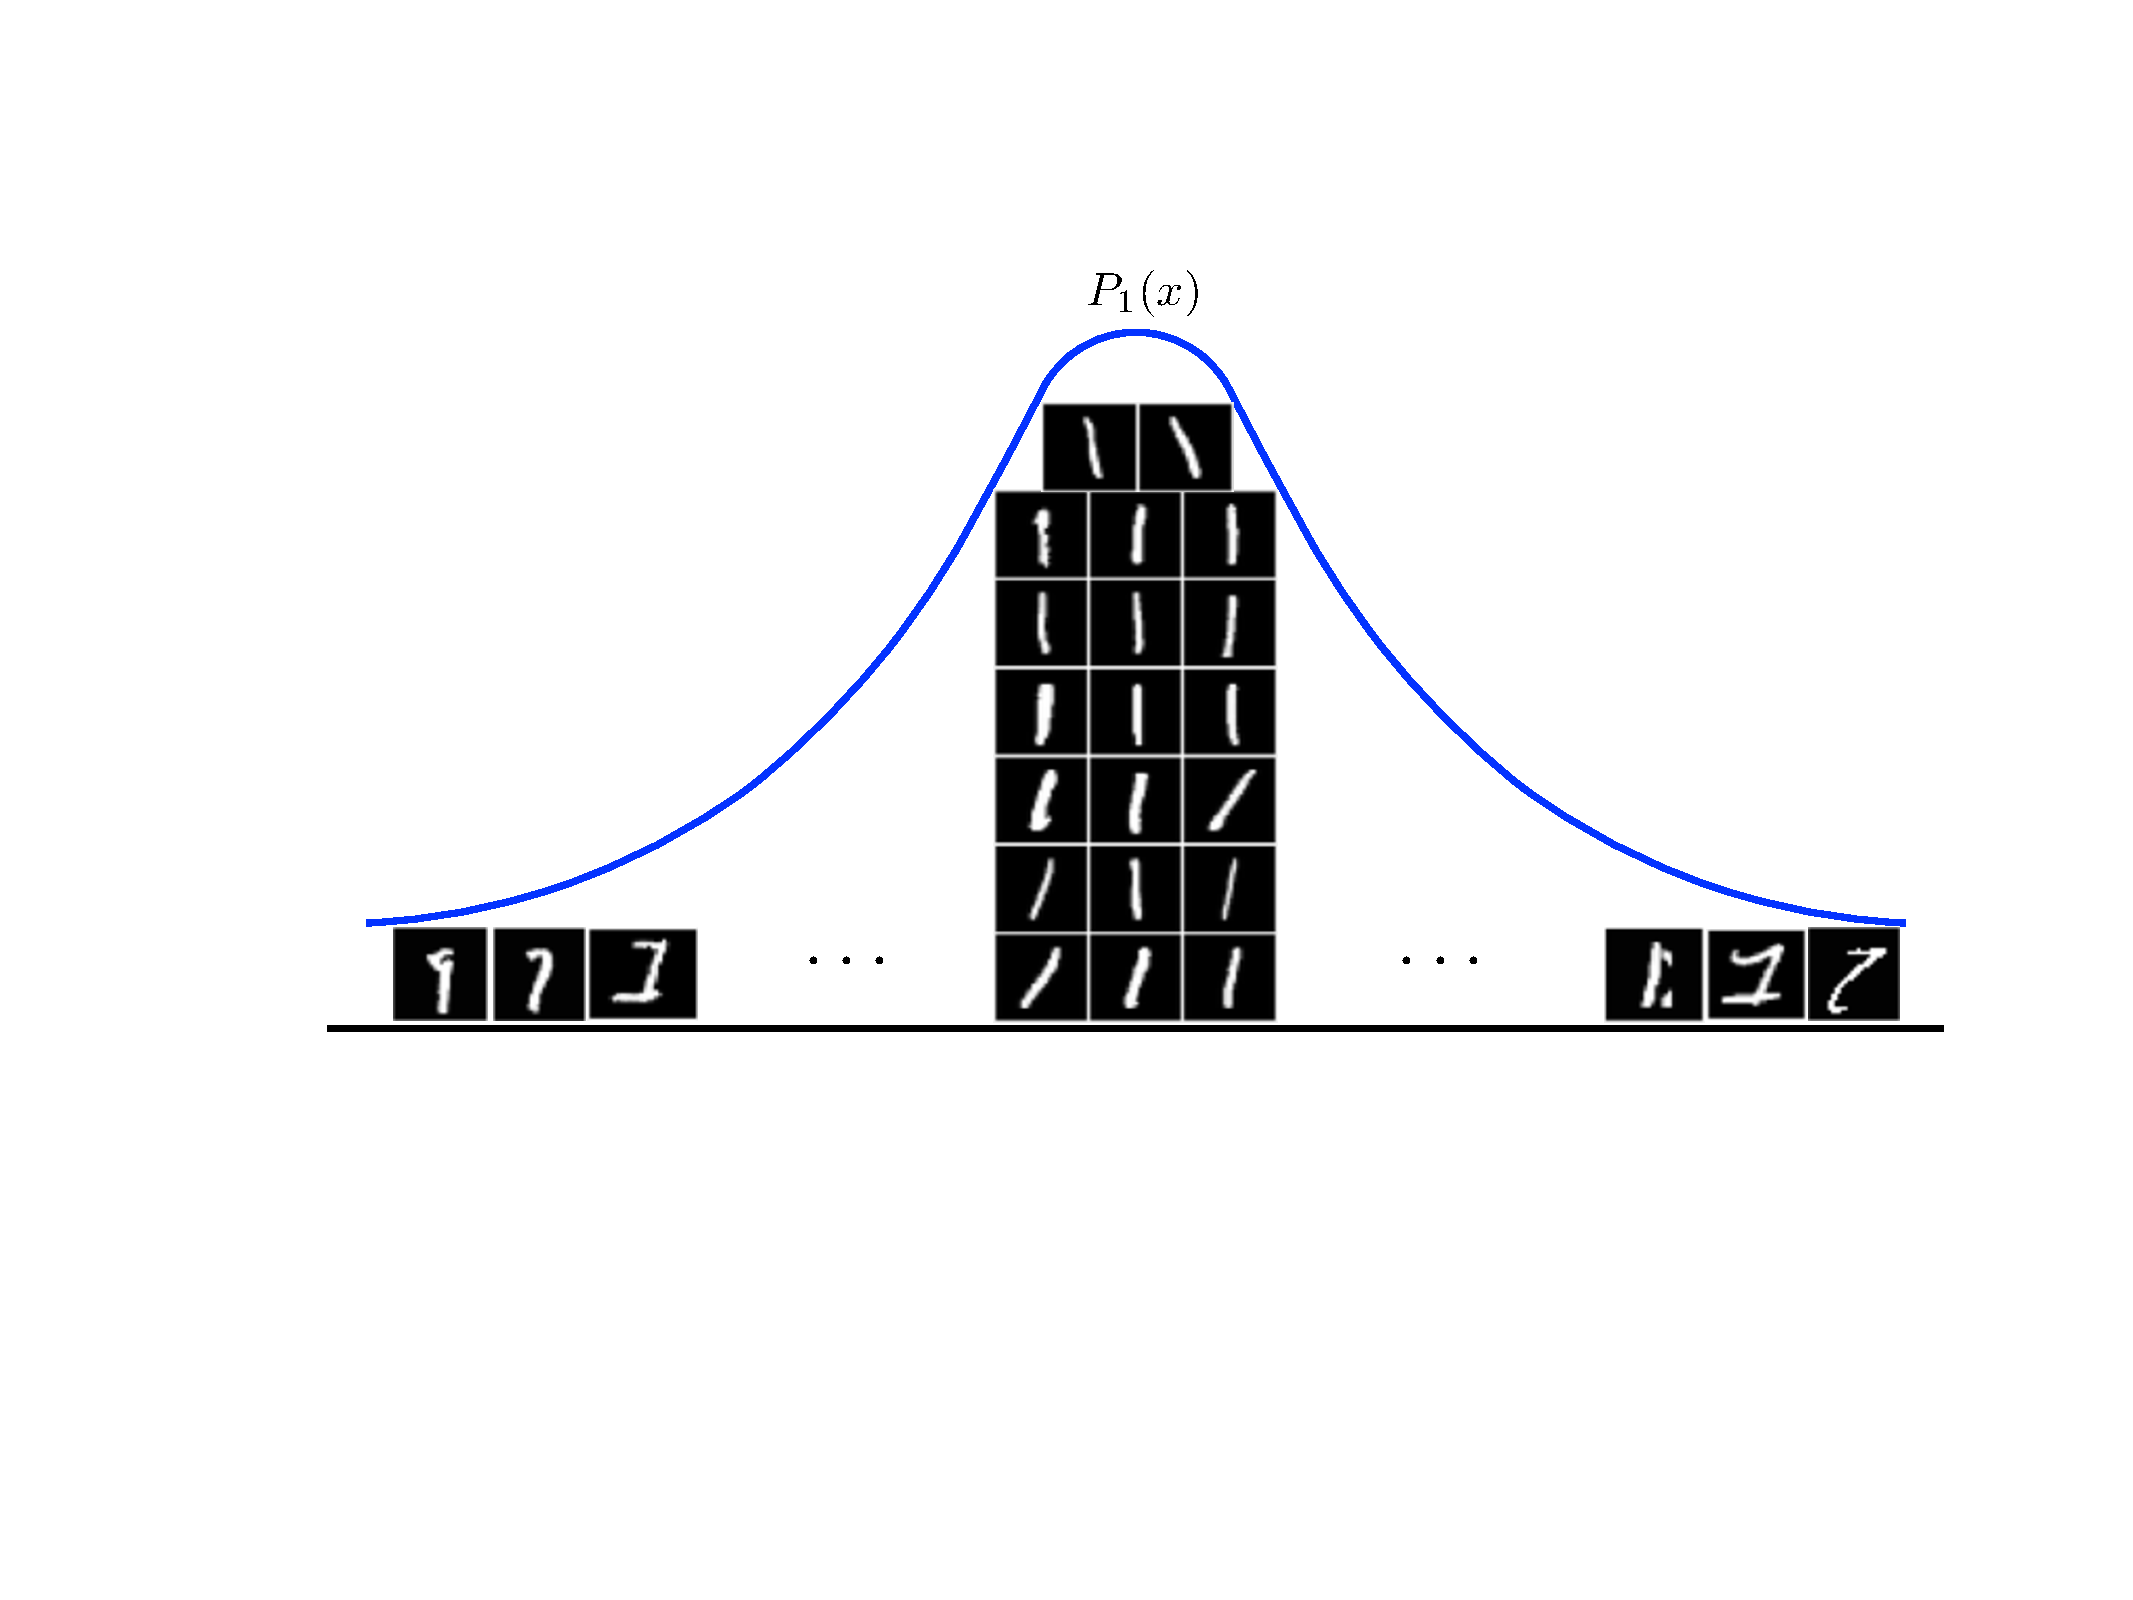
\includegraphics[scale=0.32]{P1x}
\caption{Illustration of the distribution $P_1(x)$ that captures our uncertainty of the variations among digit $1$.}
\label{fig:P1x}
\end{figure}

The distributions $P_j$ are imperfect models of the digits. Nevertheless, since they are concentrated around good images of each digit, they are still a useful representation of our knowledge. At this point it is still not clear where we get the distributions $P_j$ from, but for the moment let us assume we have them.

With this setup, we can phrase the digit classification problem in terms of balls and bins as follows: We have $10$ bins, each one corresponds to a digit. Within each bin we have all possible balls (images) corresponding to that bin (digit). We assume the images within bin $j$ are distributed according to the probability distribution $P_j$, which means the images in bin $j$ are more likely to have a digit $j$ written in them. Then we are given an image which was taken from one of the bins (the image has a digit written in it), but we don't know which one, and our task is to guess which bin the image was likely to have come from (which digit the image corresponds to).

\begin{figure}[h!]
\centering
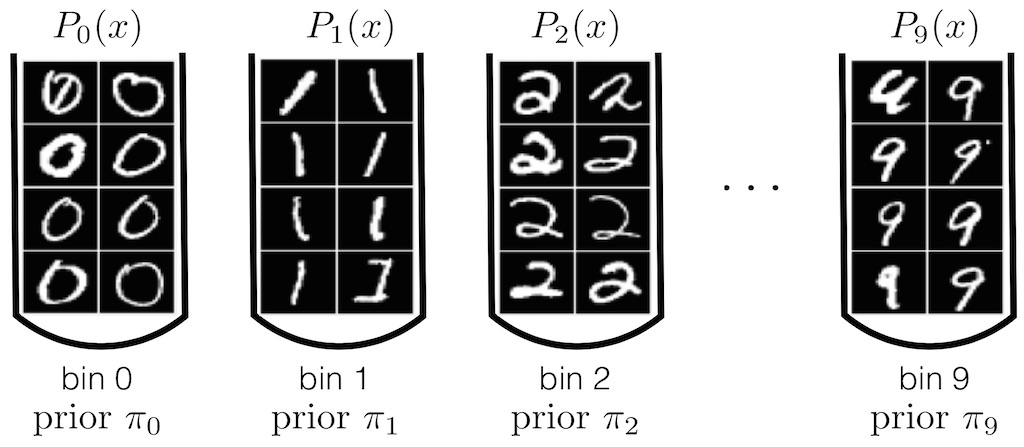
\includegraphics[scale=0.25]{ballsbins}
\caption{Balls and bins analogy of digit classification. Balls are the images, and bins are the digits.}
\label{fig:ballsbins}
\end{figure}



%%%%%%%%%%%%%%%%%%%%%%%
\subsection*{Classification as inference}

Let us assume we have a prior distribution over the bins. If $y$ denotes the bin label, then we write the prior probability distribution as
$$P(y = j) = \pi_j, ~~~~~ j \in \{0,1,\dots,9\}.$$
The prior distribution $(\pi_0,\dots,\pi_9)$ represents our initial belief on the distribution of the digits before we see any images. For example, we may believe that all $10$ digits are equally likely to appear, in which case $\pi_0 = \pi_1 = \cdots = \pi_9 = \frac{1}{10}$. Or maybe for some reason we believe that the digit $1$ appears more often than any other digits, say for example $\pi_1 = 0.3$, $\pi_2 = 0.15$, and so on.\footnote{There is an interesting justification of this called Benford's law, which states that the number 1 appears as the first significant digit more often than any other numbers. This is closely related to Zipf's law, which we will discuss in the next lecture.} But for the moment let us assume we have some prior distribution.

As noted before, we assume that within each bin $j$, the images are distributed according to $P_j$. Thus, $P_j(x)$ is the conditional probability of generating image $x$ given that the digit is $j$:
$$P(x \mid y = j) = P_j(x).$$
Now suppose we are given an image $x$. How do we decide which bin the image came from? Just like in the original balls and bins problem, we apply Bayes' rule to compute the posterior probability of each bin after having observed $x$:
\begin{align}\label{Eq:BayesBin}
P(y = j \mid x) ~=~ \frac{P(y = j) \cdot P(x \mid y = j)}{P(x)} ~=~ \frac{\pi_j \, P_j(x)}{\sum_{i=0}^9 \pi_i \, P_i(x)}.
\end{align}
In the second equality above we have used the total probability rule:
\begin{align*}
P(x) &= P(y = 0) \cdot P(x \mid y = 0) \:+\: P(y = 1) \cdot P(x \mid y = 1) \:+\: \cdots \:+\: P(y = 9) \cdot P(x \mid y = 9) \\
&= \pi_0 \, P_0(x) \:+\: \pi_1 \, P_1(x) \:+\: \cdots \:+\: \pi_9 \, P_9(x).
\end{align*}

Now that we have the posterior distribution, how should we decide which digit to classify $x$ to? The answer is simple: Choose the digit that maximizes the posterior probability! That is, classify $x$ to the digit:
\begin{align}\label{Eq:MAP1}
h(x) = \arg\max_j \; P(y = j \mid x)
\end{align}
(here ``$\arg \max_j$'' means we are taking the argument $j$ that maximizes the expression $P(y = j \mid x)$).

\begin{figure}[h!]
\centering
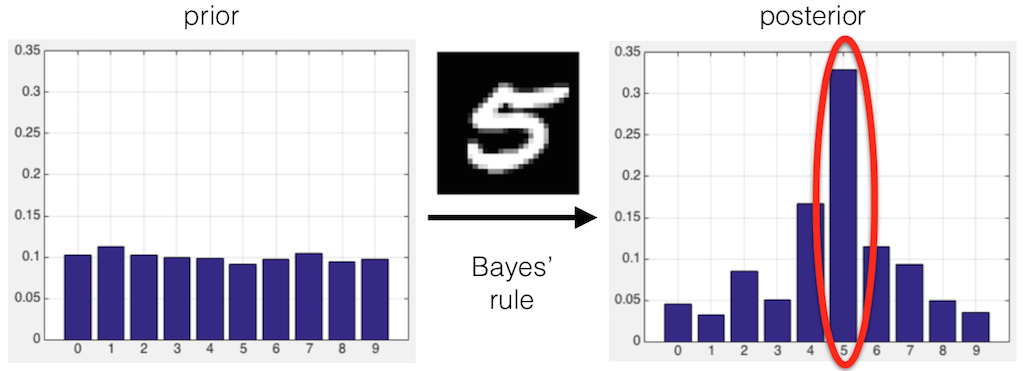
\includegraphics[scale=0.55]{priorposterior}
\caption{Updating belief by Bayes' rule after seeing image $x$. We classify $x$ to the bin with highest posterior.}
\label{fig:priorposterior}
\end{figure}

Recall that the posterior distribution~\eqref{Eq:BayesBin} represents our updated belief about the digits after seeing the image $x$. So the rule~\eqref{Eq:MAP1} is doing a simple and reasonable thing: If after seeing $x$ we believe that digit $j$ is more likely than any other digits, then we should use that digit $j$ as our guess to what number is written in $x$.

Notice from the Bayes' rule calculation~\eqref{Eq:BayesBin} that the denominator $P(x)$ does not depend on $j$. Therefore, we can omit $P(j)$ from the maximization problem over $j$ in~\eqref{Eq:MAP1}, so we can equivalently write:
\begin{align}\label{Eq:MAP2}
h(x) = \arg\max_j \; \pi_j \, P_j(x).
\end{align}
The estimator in~\eqref{Eq:MAP1} and~\eqref{Eq:MAP2} is called the {\em Bayes optimal} estimator. It is also known as the {\em maximum a posteriori (MAP)} estimator, i.e., the one that maximizes the posterior distribution.



%%%%%%%%%%%%%%
\subsection*{Estimating the distributions}

We have reduced the problem of classification into inference: To classify an image $x$, we only need to calculate the prior $\pi_j$ and the conditional probability $P_j(x)$ for all digits $j \in \{0,1,\dots,9\}$, and find the one that maximizes their product~\eqref{Eq:MAP2}. So if we know the prior distribution $\pi_j$ and all the conditional distributions $P_j$, then we are done. But where do they come from?

One way to obtain these distributions is to learn them from the data. Typically, in a machine learning problem we have access to some training data that we can use to train our model, and some test data to test the performance of our model. The MNIST dataset that we are using provides 60000 training examples (where each example consists of a pair $(x,y)$ of an image and the corresponding digit) and 10000 test images.

\medskip
{\bf Estimating the prior.}~
Recall that the prior probability $\pi_j = P(y = j)$ is our initial belief about the distribution of the digits. Suppose we are given $n$ training examples ($n = 60000$ in our case). We divide them into $10$ parts based on the digits in the images. Then we estimate the prior probability $\pi_j$ by:
\begin{align}\label{Eq:PriorEst}
\hat \pi_j = \frac{n_j}{n}
\end{align}
where $n_j$ is the number of examples having digit $j$. Intuitively, we are thinking of the training examples as random samples taken from the underlying distribution that generates the digits and the images. If the probability of getting digit $j$ is $\pi_j$, then among $n$ samples we expect to get $n_j = n \pi_j$ images with digit $j$, so our estimate for $\pi_j$ should be $\hat \pi_j = \frac{n_j}{n}$. Notice that $n_0 + n_1 + \cdots + n_9 = n$, so $\hat \pi_0 + \hat \pi_1 + \cdots + \hat \pi_9 = 1$, which means our estimate $(\hat \pi_0, \hat \pi_1, \dots, \hat \pi_9)$ forms a valid probability distribution.

The prior estimate from the MNIST dataset is as follows (these are displayed on the left plot in Figure~\ref{fig:priorposterior}):
\begin{center}
\begin{tabular}{c | c c c c c c c c c c}
$j$ & 0 & 1 & 2 & 3 & 4 & 5 & 6 & 7 & 8 & 9 \\
\hline
$\hat \pi_j$ (\%) &  9.87 & 11.24 & 9.93 & 10.22 & 9.74 & 9.03 & 9.86 & 10.44 & 9.75 & 9.92
\end{tabular}
\end{center}

\medskip
{\bf Estimating the conditional.}
We see that estimating the prior is easy. But estimating the conditional distribution $P_j(x) = P(x \mid y = j)$ is more difficult. In the MNIST dataset, each image $x$ is grayscale (each pixel value is between $0$ and $1$) and has size $28 \times 28$ pixels. So each image $x$ is a point in the ($28 \times 28 = $) $784$-dimensional space, $x \in [0,1]^{784}$. What kind of distribution should we use to represent $P_j(x)$? In particular, how should we try to model the distribution of the images of digit $j$?

The important idea is: We don't have to model the distribution of the digits accurately. It turns out that we can use a very simple model that is perhaps unrealistic, but easy to learn. Then with the help of Bayes' rule and the formalism of inference, we can still use this simple model to obtain a good performance in our digit classification task. In the rest of this note, we will see two simple models:
\begin{enumerate}
  \item {\bf Naive Bayes}: Assume $P_j(x)$ is a product of independent coin flips. This means we assume each pixel value is independent of all other pixels.
  
  \item {\bf Gaussian model}: Assume $P_j(x)$ is a multivariate Gaussian distribution. This allows us to model the correlation between pixel values, but still keeping the model simple and easy to learn.
\end{enumerate}



%%%%%%%%%%%%%%
\subsection*{Naive Bayes}

Let us assume for now that we have binary images. That is, we convert our grayscale image $x \in [0,1]^{784}$ into a binary image $x \in \{0,1\}^{784}$ by thresholding each pixel value (if $x_i \ge \frac{1}{2}$, then assign it to $x_i = 1$, otherwise assign it to $x_i = 0$). Then for each digit $j \in \{0,1,\dots,9\}$, our conditional distribution $P_j(x)$ is a probability distribution over the discrete space $\{0,1\}^{784}$, which has $2^{784}$ elements. So a general distribution over $\{0,1\}^{784}$ requires specifying $2^{784}$ numbers that sum up to $1$, and that is a very large number of parameters.

In the Naive Bayes model, we make an assumption that greatly simplifies the number of parameters: We assume that within each digit, the individual pixel values are independent $\{0,1\}$-random variables. This means the probability distribution $P_j$ over $x = (x_1, x_2, \dots, x_{784}) \in \{0,1\}^{784}$ factorizes into a product:
\begin{align}\label{Eq:PjNaive}
P_j(x) = P_{j1}(x_1) \cdot P_{j2}(x_2) \cdots P_{j,784}(x_{784}).
\end{align}
Each individual distribution $P_{ji}(x_i)$ is a probability distribution over the value of the $i$-th pixel $x_i \in \{0,1\}$. We can think of each $P_{ji}$ as a biased coin flip with bias $p_{ji}$:
\begin{align*}
P_{ji}(x_i = 1) = p_{ji}, ~~~~~~~~~~~~ P_{ji}(x_i = 0) = 1-p_{ji},
\end{align*} 
which we can more concisely write as:
\begin{align}\label{Eq:Pji}
P_{ji}(x_i) = p_{ji}^{x_i} \, (1-p_{ji})^{1-x_i}, ~~~~ x_i \in \{0,1\}.
\end{align}
So now the distribution $P_j(x)$ in~\eqref{Eq:PjNaive} only has $784$ parameters $(p_{j1}, p_{j2}, \dots, p_{j,784})$. Moreover, these parameters are easy to learn: Estimating each $p_{ji}$ is the same problem as estimating the bias of a coin, which we know how to do.

Specifically, fix a digit $j \in \{0,1,\dots,9\}$ and a pixel $i \in \{1,2,\dots,784\}$. Out of $n$ training examples, let $n_j$ be the number of examples with digit $j$. Among these $n_j$ examples with digit $j$, let $n_{ji}$ be the number of examples having $x_i = 1$. Then we estimate $p_{ji}$ by
\begin{align}\label{Eq:pjiEst}
\hat p_{ji} = \frac{n_{ji}}{n_j}.
\end{align}
Recall the intuition: We are thinking of the $n_j$ examples as random samples drawn from the underlying (conditional) distribution of images with digit $j$. If the probability of pixel $i$ being on ($x_i=1$) is equal to $p_{ji}$, then among these $n_j$ samples we expect to see $n_{ji} = n_j p_{ji}$ images with $x_i = 1$. Therefore, our estimate for $p_{ji}$ should be $\hat p_{ji} = \frac{n_{ji}}{n_j}$.

\medskip
{\bf Remark:}~The estimator~\eqref{Eq:pjiEst} is problematic if $n_{ji} = 0$ (we always see $x_i = 0$, in which case $\hat p_{ji} = 0$) or $n_{ji} = n_j$ (we always see $x_i = 1$, in which case $\hat p_{ji} = 1$). This is because we want to use the estimator $\hat p_{ji}$ to make predictions for a future image $x$. If in our training examples we always see $x_i = 1$ ($n_{ji} = n_j$), then by taking $\hat p_{ji} = 1$ we are saying that all future values of $x_i$ will always be equal to $1$. However, it can also be the case that the $n_j$ examples that we see by random chance happen to be all $x_i = 1$, even if the true value of $p_{ji}$ is $< 1$, in which case it is possible for the future values of $x_i$ to be $0$. So to hedge our bet, in practice we usually want to use what is called {\em Laplace smoothing}:
\begin{align}\label{Eq:pjiLaplace}
\tilde p_{ji} = \frac{n_{ji}+1}{n_j+2}.
\end{align}
This has the effect that even if $n_{ji} = 0$ or $n_{ji} = n_j$, the estimator $\tilde p_{ji}$ will be strictly $> 0$ and $< 1$. An interpretation of the Laplace smoothing~\eqref{Eq:pjiLaplace} is that it is as if we have two additional examples with digit $j$: one example with $x_i = 0$, and one example with $x_i = 1$.


\medskip
{\bf Naive Bayes classifier.}~With the ingredients above, we can summarize the Naive Bayes classifier as follows. The data space is the set of all possible binary images, $\X = \{0,1\}^{784}$. The label space is the set of all possible digits, $\Y = \{0,1,\dots,9\}$. From the training data, we estimate:
\begin{itemize}
  \item Prior probability $(\pi_0, \pi_1, \dots, \pi_9)$ following~\eqref{Eq:PriorEst}.
  \item Conditional probability $p_{ji}$ for all digits $0 \le j \le 9$ and pixels $1 \le i \le 784$, following~\eqref{Eq:pjiEst} or~\eqref{Eq:pjiLaplace}.
\end{itemize}
Given an image $x = (x_1,\dots,x_{784}) \in \{0,1\}^{784}$, we can compute its conditional likelihood given digit $j$ as:
\begin{align*}
P_j(x) ~=~ \prod_{i=1}^{784} P_{ji}(x_i) ~=~ \prod_{i=1}^{784} \, p_{ji}^{x_i} (1-p_{ji})^{1-x_i}.
\end{align*}
In the first equality above we use the Naive Bayes assumption~\eqref{Eq:PjNaive}, and in the second equality we use~\eqref{Eq:Pji}. Then we use our inference framework and classify image $x$ to the digit given by the MAP estimator~\eqref{Eq:MAP2}:
\begin{align*}
h(x) ~=~ \arg\max_j \; \pi_j \, P_j(x)
~=~ \arg\max_j \; \pi_j \, \prod_{i=1}^{784} \: p_{ji}^{x_i} \, (1-p_{ji})^{1-x_i}.
\end{align*}
But notice that in the calculation above we are multiplying many small numbers, so the resulting product will be very small, and may be rounded down to $0$ if the value is smaller than the limit of precision of the computer; this is called underflow. To avoid underflow, we can maximize the logarithm instead:\footnote{Note that $z \mapsto \log z$ is a monotonically increasing function, so maximizing an expression $f(j)$ is equivalent to maximizing its logarithm $\log f(j)$. The maximum value will be different, but the argument that achieves the maximum will be the same.}
\begin{align*}
h(x)
~=~ \arg\max_j \; \log \pi_j + \sum_{i=1}^{784} \, \Big( x_i \, \log p_{ji} + (1-x_i) \log (1-p_{ji}) \Big).
\end{align*}
This is the entire Naive Bayes classifier, a very simple algorithm. Let's now see how well it works.

\medskip
{\bf Naive Bayes on MNIST.}~When we apply the Naive Bayes classifier to the MNIST dataset, we obtain 15.4\% error rate on 10000 test data (i.e., we misclassified 1540 images). This is already a pretty good performance, because there are $10$ classes, so if we were to guess randomly, then we would expect an error rate of 90\%. Figure~\ref{fig:naive_mis} shows some examples of the images that are misclassified.

\begin{figure}[h!]
\centering
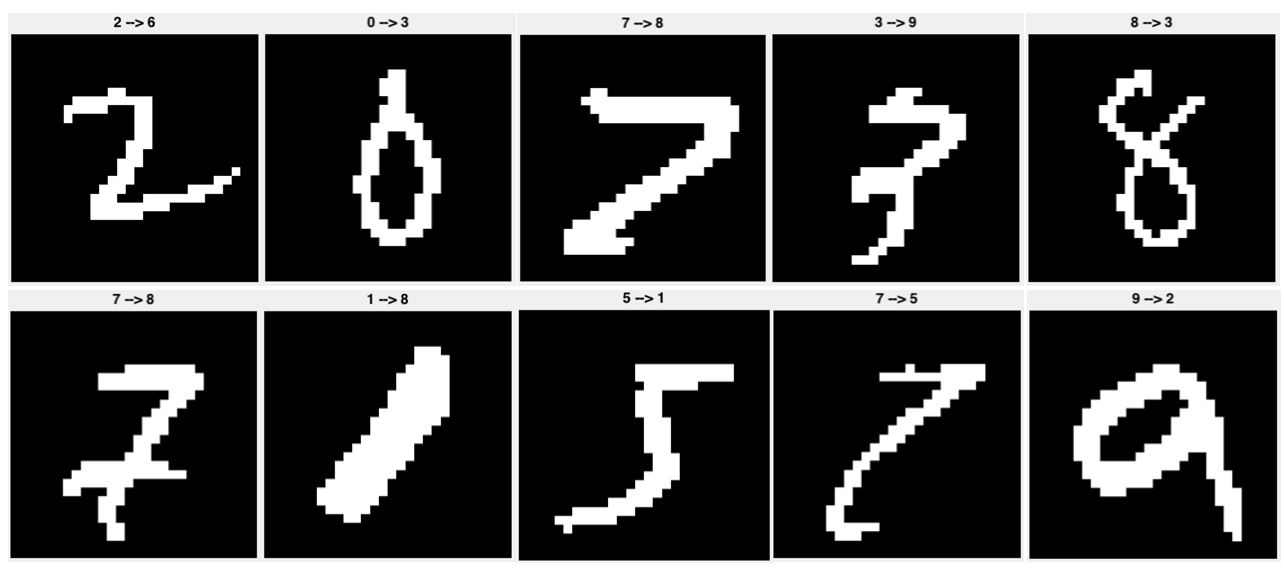
\includegraphics[scale=0.4]{naive_mis}
\caption{Examples of test images that are misclassified by Naive Bayes.}
\label{fig:naive_mis}
\end{figure}

Let us examine the Naive Bayes model more closely. Figure~\ref{fig:meannaive} shows the mean vectors for each digit, namely, the estimated values of $p_{ji}$ (so for each digit $j$, we render the estimated values $(p_{j1}, p_{j2}, \dots,$ $p_{j,784})$ as a grayscale $28 \times 28$ image). We can also generate samples from the Naive Bayes model we have trained. That is, for each digit $j$, we can generate a sample $x = (x_1,\dots,x_{784}) \in \{0,1\}^{784}$ from the conditional distribution $P_j$ by sampling each pixel $x_i$ independently from the distribution $P_{ji}$ (i.e., $x_i$ is a biased coin flip with bias $p_{ji}$). Figure~\ref{fig:naivesamples} show some samples generated from the model. The first two rows are ordered based on the digits, while the last two rows are arranged in an arbitrary order. Can you still recognize the digits?


\begin{figure}[h!]
\centering
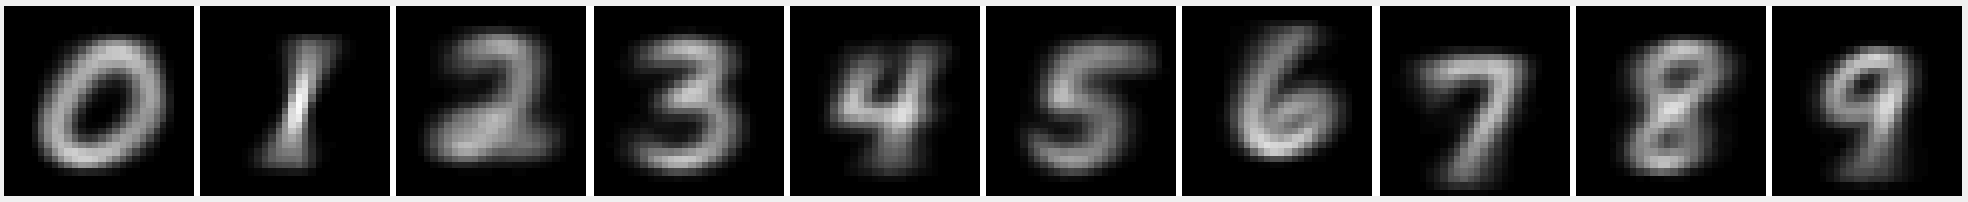
\includegraphics[scale=0.46]{meannaive}
\caption{Mean vectors for each digit (the estimated $p_{ji}$'s).}
\label{fig:meannaive}
\end{figure}

\begin{figure}[h!]
\centering
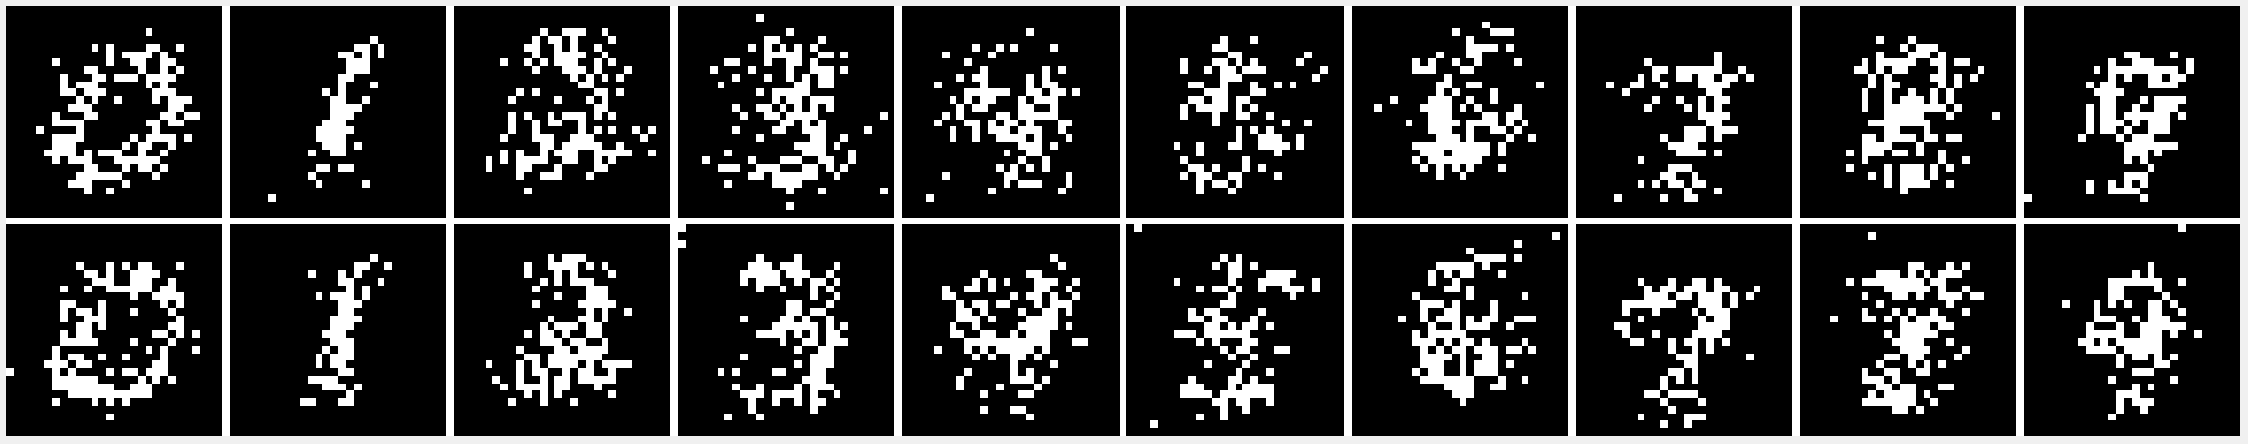
\includegraphics[scale=0.4]{naivesamples_ordered} \\
\vspace{4pt}
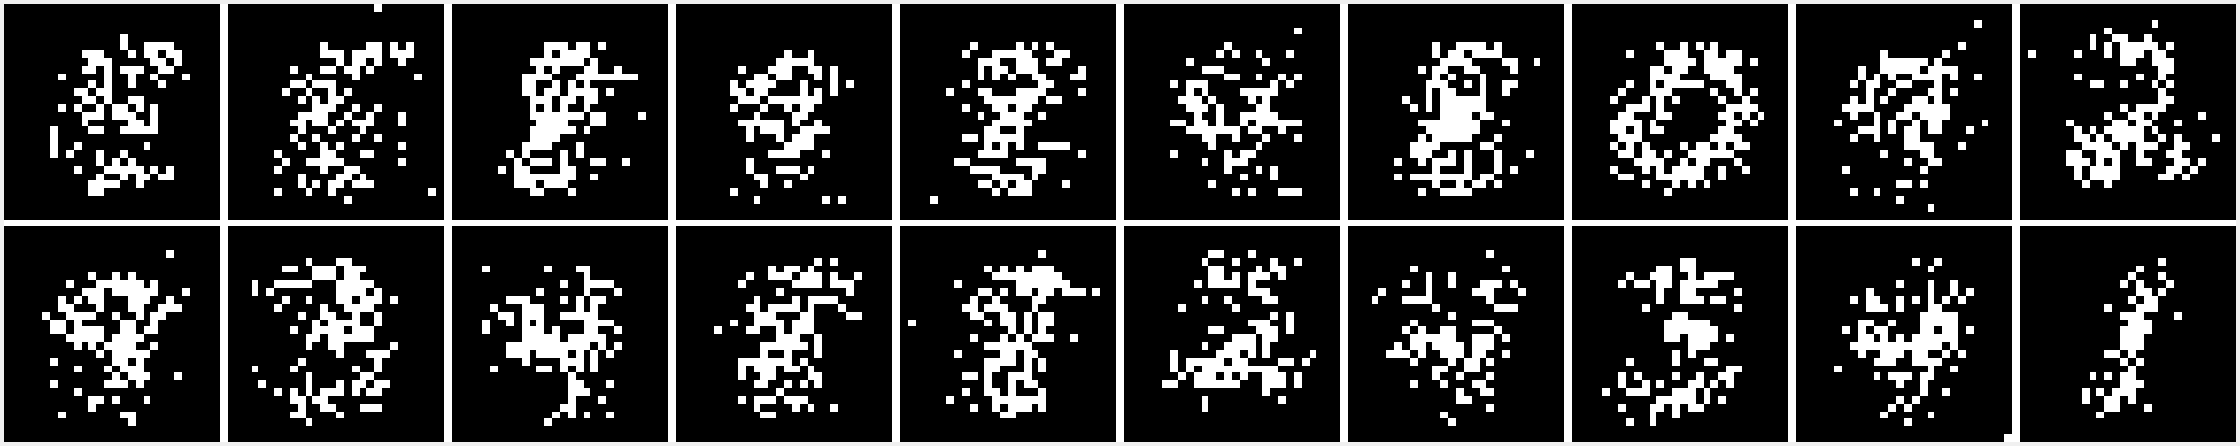
\includegraphics[scale=0.4]{naivesamples_random}
\caption{Some samples generated from the trained Naive Bayes model.}
\label{fig:naivesamples}
\end{figure}

From Figure~\ref{fig:naivesamples} we see that the samples generated from the Naive Bayes model don't look like the training data that we started with (Figure~\ref{fig:digits} and Figure~\ref{fig:digits2}). Some of the samples still look like digits, but others are not recognizable. This shows that the Naive Bayes model does not really capture the true characteristics of the digits. In particular, the independence assumption is clearly dubious, because from the training images we see that the black and white pixels tend to appear in groups, so if a pixel is surrounded by many white pixels then it is also more likely to be white, and vice versa. Yet with this very simple, unrealistic model we are able to achieve a pretty good performance.

We can now try to improve upon this model and try to build a more accurate representation of the digits, thereby obtaining better performance, but at the cost of a more complex model and more expensive learning procedure. This is a general trade-off between model accuracy and complexity that we have to make in many problems.



%%%%%%%%%%%%%%
\subsection*{Gaussian model\footnote{This section requires linear algebra beyond the scope of this class, so this section is optional and only for your own interest.}}

The next model we will look at is the Gaussian model. Here we are treating the grayscale image $x \in [0,1]^{784}$ as a vector in the $784$-dimensional real space, $x \in \R^{784}$, and we are assuming that within each digit, the images are distributed according to a multivariate Gaussian distribution. This has the advantage that we are also modeling the correlation between different pixel values, while still keeping the model relatively simple and easy to learn.


\subsubsection*{A brief overview of multivariate Gaussian}

What do multivariate Gaussian distributions look like? Recall that the univariate (one-dimensional) Gaussian distribution $N(\mu,\sigma^2)$ is specified by a mean value $\mu \in \R$ and variance $\sigma^2 > 0$. The density of the univariate Gaussian distribution $N(\mu,\sigma^2)$ is given by:
\begin{align}\label{Eq:Gaussian1}
p(x) = \frac{1}{\sqrt{2\pi \sigma^2}} \: \exp\left(-\frac{(x-\mu)^2}{2\sigma^2} \right), ~~~~~~~~ x \in \R.
\end{align}
Figure~\ref{fig:gaussian1} shows the plot of the density function $p(x)$. Notice the characteristic bell-shaped curve centered around the mean $\mu$ and rapidly decreasing as $x$ moves away from $\mu$. This is because the density function $p(x)$ is an exponential function of a negative quadratic function of $x$, as we can see from~\eqref{Eq:Gaussian1} above.

\begin{figure}[h!]
\centering
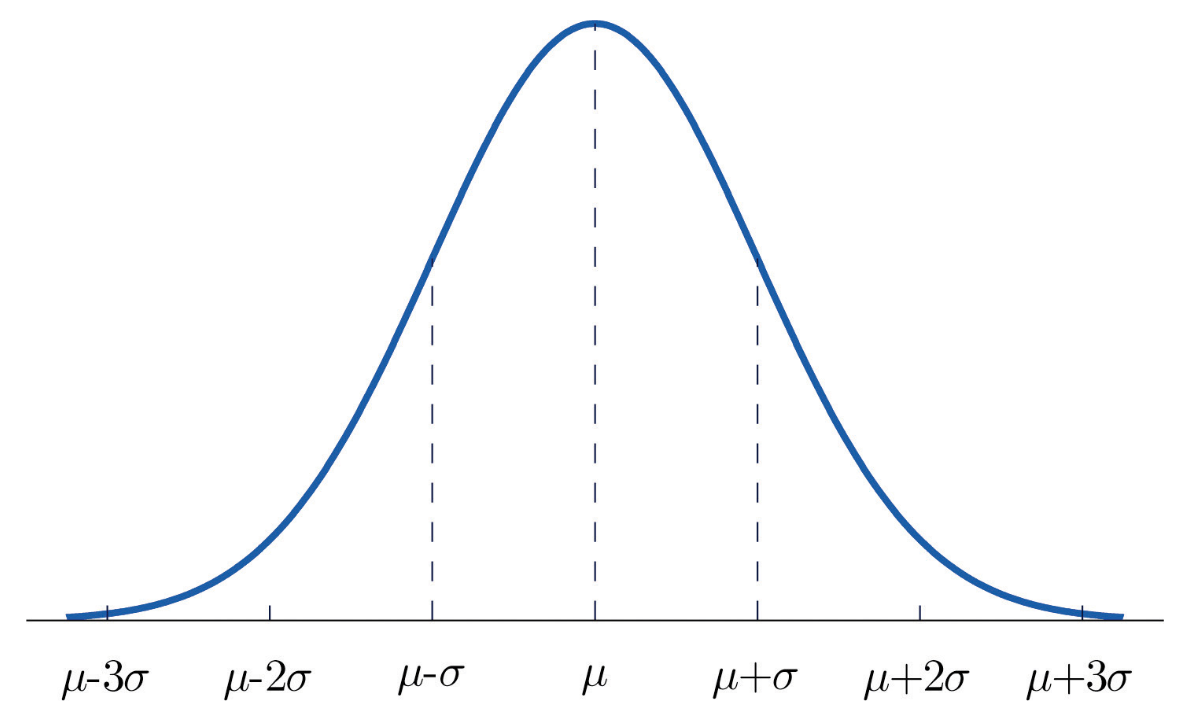
\includegraphics[scale=0.3]{unigaussian}
\caption{Plot of density function of the univariate Gaussian distribution $N(\mu,\sigma^2)$.}
\label{fig:gaussian1}
\end{figure}

\smallskip
{\bf Bivariate Gaussian: same variance.}~
We now consider bivariate (two-dimensional) Gaussian. We start with the simplest case: Let's take two independent univariate Gaussian random variables $X_1 \sim N(\mu_1, \sigma^2)$ and $X_2 \sim N(\mu_2, \sigma^2)$, so they have mean values $\Ex{X_1} = \mu_1$ and $\Ex{X_2} = \mu_2$, and the same variance $\Var{X_1} = \Var{X_2} = \sigma^2$. We combine $X_1$ and $X_2$ into a column vector $X$, and $\mu_1$ and $\mu_2$ into a column vector $\mu$:
\begin{align*}
X = \begin{pmatrix} X_1 \\ X_2 \end{pmatrix}, ~~~~~~~~~~~~ \mu = \begin{pmatrix} \mu_1 \\ \mu_2 \end{pmatrix}.
\end{align*}
Now we have a two-dimensional random variable $X \in \R^2$, which has a bivariate Gaussian distribution with mean vector $\Ex{X} = \mu$. The density function of $X$ is the joint density of $X_1$ and $X_2$:
\begin{align*}
p(x) ~=~ p(x_1, x_2) ~=~ p_1(x_1) \cdot p_2(x_2)
\end{align*}
where in the last equality we are using the property that the joint density of independent random variables is the product of their densities. Now plugging in the univariate Gaussian density for $X_1 \sim N(\mu_1, \sigma^2)$ and $X_2 \sim N(\mu_2, \sigma^2)$, we get that the density function of $X$ is:
\begin{align}
p(x) ~&=~ \left\{\frac{1}{\sqrt{2\pi \sigma^2}} \: \exp\left(-\frac{(x_1-\mu_1)^2}{2\sigma^2} \right) \right\} \cdot \left\{\frac{1}{\sqrt{2\pi \sigma^2}} \: \exp\left(-\frac{(x_2-\mu_2)^2}{2\sigma^2} \right) \right\}  \notag \\
~&=~ \frac{1}{2\pi \sigma^2} \exp \left(- \frac{\|x - \mu\|^2}{2\sigma^2} \right)  \label{Eq:Gaussian2sphere}
\end{align}
where we have used the notation $\|x-\mu\|$ to denote the norm of the vector $x-\mu \in \R^2$:
\begin{align*}
\|x-\mu\| ~=~ \sqrt{(x_1-\mu_1)^2 \:+\: (x_2-\mu_2)^2}.
\end{align*}
From~\eqref{Eq:Gaussian2sphere}, we see that the density $p(x)$ only depends on the distance from the point $x$ to the mean vector $\mu$, so the density function $p(x)$ is rotationally symmetric around the mean $\mu$.\footnote{We have seen this property in Note~20 when proving that the sum of two independent normal random variables is also normal.} Figure~\ref{fig:gaussian2sphere} shows the contour plot of the density function~\eqref{Eq:Gaussian2sphere}. Each green circle in Figure~\ref{fig:gaussian2sphere} has the same density value (but the density decreases as the circle gets larger), so this special case is also called the {\em spherical Gaussian distribution}.


\begin{figure}[h!]
\centering
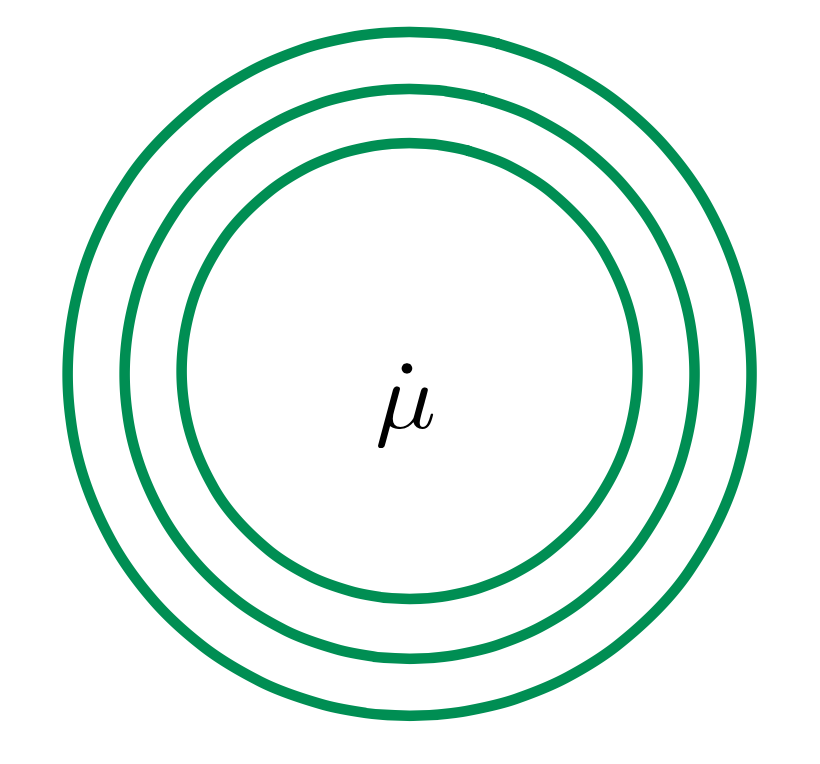
\includegraphics[scale=0.25]{sphericalGaussian}
\caption{Contour plot of density function $p(x)$ of the spherical two-dimensional Gaussian distribution~\eqref{Eq:Gaussian2sphere}.}
\label{fig:gaussian2sphere}
\end{figure}

\smallskip
{\bf Bivariate Gaussian: different variances.}~
Consider two independent univariate Gaussian random variables $X_1 \sim N(\mu_1, \sigma_1^2)$ and $X_2 \sim N(\mu_2, \sigma_2^2)$, so now they have different means $\Ex{X_1} = \mu_1$, $\Ex{X_2} = \mu_2$, and different variances $\Var{X_1} = \sigma_1^2$, $\Var{X_2} = \sigma_2^2$. As before, we collect $X_1$ and $X_2$ into a vector $X$; $\mu_1$ and $\mu_2$ into a vector $\mu$; and now we also collect $\sigma_1^2$ and $\sigma_2^2$ into a matrix $\Sigma$:
\begin{align*}
X = \begin{pmatrix} X_1 \\ X_2 \end{pmatrix}, ~~~~~~~~~~~~ \mu = \begin{pmatrix} \mu_1 \\ \mu_2 \end{pmatrix},
~~~~~~~~~~~~ \Sigma = \begin{pmatrix} \sigma_1^2 & 0 \\ 0 & \sigma_2^2 \end{pmatrix}.
\end{align*}

Notice that since $X_1$ and $X_2$ are independent, they have zero covariance:
\begin{align*}
{\rm Cov}(X_1, X_2) = \Ex{(X_1 - \mu_1)(X_2 - \mu_2)} = 0.
\end{align*}
So the off-diagonal entries of the matrix $\Sigma$, which are equal to $0$, are actually the covariance of $X_1$ and $X_2$. Then the vector $X$ has a two-dimensional Gaussian distribution with mean vector $\Ex{X} = \mu$ and diagonal covariance matrix $\Sigma$, namely:
\begin{align*}
{\rm Cov}(X) ~=~ \begin{pmatrix} \Var{X_1} & {\rm Cov}(X_1, X_2) \\ {\rm Cov}(X_2, X_1) & \Var{X_2} \end{pmatrix}
~=~ \begin{pmatrix} \sigma_1^2 & 0 \\ 0 & \sigma_2^2 \end{pmatrix} 
~=~ \Sigma.
\end{align*}
The density of $X$ is given by the joint density of $(X_1,X_2)$, which is the product of their individual densities:
\begin{align}
p(x) ~&=~ \left\{\frac{1}{\sqrt{2\pi \sigma_1^2}} \: \exp\left(-\frac{(x_1-\mu_1)^2}{2\sigma_1^2} \right) \right\} \cdot \left\{\frac{1}{\sqrt{2\pi \sigma_2^2}} \: \exp\left(-\frac{(x_2-\mu_2)^2}{2\sigma_2^2} \right) \right\}  \notag \\
~&=~ \frac{1}{2\pi \, \sigma_1 \, \sigma_2} \exp \left(- \frac{(x_1 - \mu_1)^2}{2 \sigma_1^2} - \frac{(x_2 - \mu_2)^2}{2\sigma_2^2} \right)   \notag \\
~&=~ \frac{1}{2\pi \, |\Sigma|^{1/2}} \exp \left(- \frac{1}{2} (x - \mu)^\top \Sigma^{-1} (x-\mu) \right)  \label{Eq:Gaussian2diagonal}
\end{align}
In the last equality above we have used the notation $|\Sigma|$ for the determinant of the matrix $\Sigma$:
$$|\Sigma| = \det(\Sigma) = \det \begin{pmatrix} \sigma_1^2 & 0 \\ 0 & \sigma^2 \end{pmatrix} = \sigma_1^2 \cdot \sigma_2^2.$$
The expression inside the exponential in~\eqref{Eq:Gaussian2diagonal} is a quadratic function in $x \in \R^2$ involving the inverse covariance matrix $\Sigma^{-1}$ (here $(x-\mu)^\top$ is a row vector that is the transpose of $(x-\mu)$):
\begin{align*}
(x - \mu)^\top \Sigma^{-1} (x-\mu)
~=~ \begin{pmatrix} x_1 - \mu_1 & x_2 - \mu_2 \end{pmatrix}
\begin{pmatrix} \frac{1}{\sigma_1^2} & 0 \\ 0 & \frac{1}{\sigma_2^2} \end{pmatrix}
\begin{pmatrix} x_1 - \mu_1 \\ x_2 - \mu_2 \end{pmatrix}
~=~ \frac{(x_1 - \mu_1)^2}{\sigma_1^2} + \frac{(x_2 - \mu_2)^2}{\sigma_2^2}.
\end{align*}

Figure~\ref{fig:gaussian2diagonal} shows the contour plot of the density function~\eqref{Eq:Gaussian2diagonal}, where now each contour is not a circle anymore, but an ellipse. We can think of the ellipses as being obtained by stretching the circles in Figure~\ref{fig:gaussian2sphere} along the axes, where the amount of stretching is proportional to the variances.

\begin{figure}[h!]
\centering
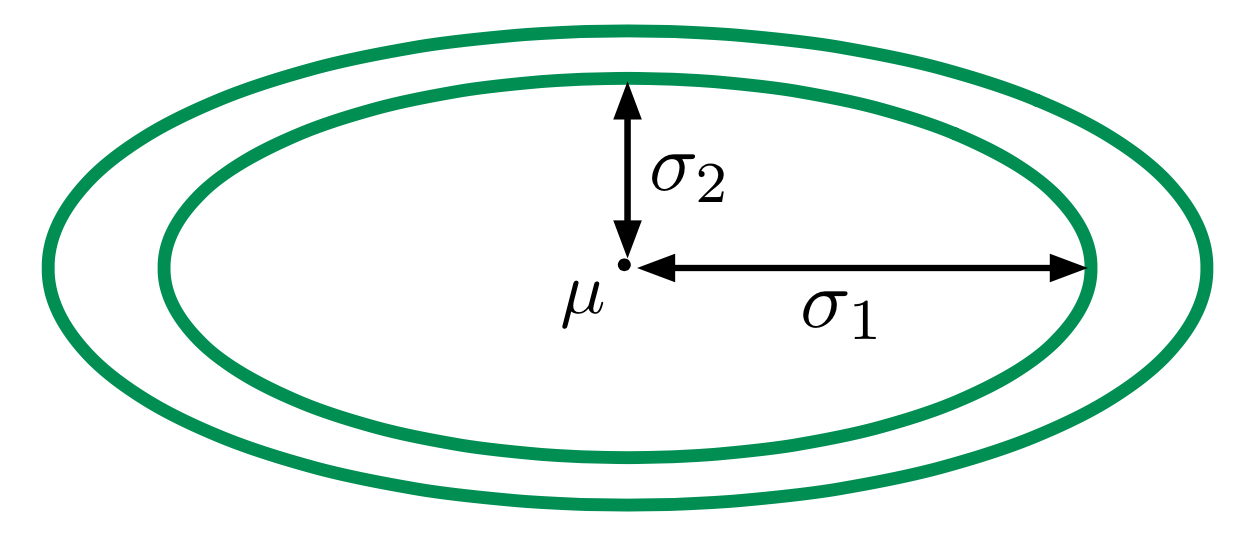
\includegraphics[scale=0.25]{diagonalGaussian}
\caption{Contour plot of density function $p(x)$ of the diagonal two-dimensional Gaussian distribution~\eqref{Eq:Gaussian2diagonal}.}
\label{fig:gaussian2diagonal}
\end{figure}

\smallskip
{\bf Bivariate Gaussian: general.}~The general bivariate Gaussian distribution $N(\mu,\Sigma)$ is specified by a mean vector $\mu \in \R^2$ and a $2 \times 2$ covariance matrix $\Sigma$. The density function is given by the same expression in~\eqref{Eq:Gaussian2diagonal}, but now with a general covariance matrix:
\begin{align}\label{Eq:Gaussian2general}
p(x) ~=~ \frac{1}{2\pi \, |\Sigma|^{1/2}} \exp \left(- \frac{1}{2} (x - \mu)^\top \Sigma^{-1} (x-\mu) \right).
\end{align}
It can be shown that the covariance matrix $\Sigma$ can be decomposed into perpendicular directions $u_1, u_2 \in \R^2$, such that $\Sigma$ only acts by scaling along each direction, namely, $\Sigma \, u_1 = \sigma_1^2 u_1$ and $\Sigma \, u_2 = \sigma_2^2 u_2$. Thus, having a general covariance $\Sigma$ is essentially the same as having a diagonal covariance matrix as in~\eqref{Eq:Gaussian2diagonal}, except that the axes are now rotated. Figure~\ref{fig:gaussian2general} shows the contour plot of the density function~\eqref{Eq:Gaussian2general}. We see that the contours are still ellipses, but oriented along the axes $u_1$ and $u_2$.

\begin{figure}[h!]
\centering
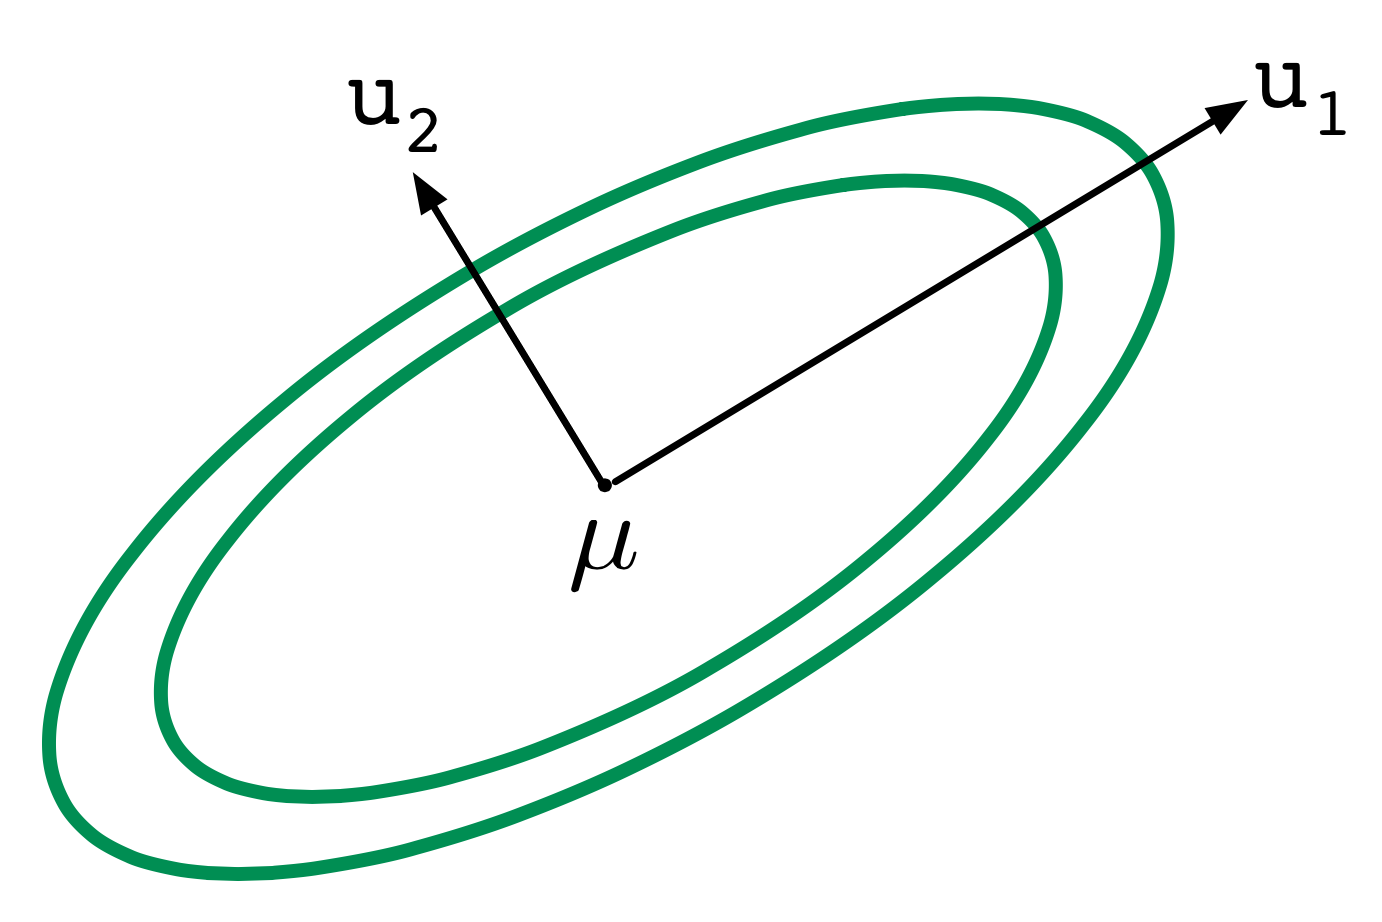
\includegraphics[scale=0.22]{generalGaussian2}
\caption{Contour plot of density function $p(x)$ of the general two-dimensional Gaussian distribution~\eqref{Eq:Gaussian2general}.}
\label{fig:gaussian2general}
\end{figure}

\smallskip
{\bf Multivariate Gaussian.}~The general multivariate Gaussian in $\R^d$ is just the high-dimensional analog of the bivariate case above. The Gaussian distribution $N(\mu,\Sigma)$ in $\R^d$ is specified by a mean vector $\mu \in \R^d$ and a $d \times d$ covariance matrix $\Sigma$. The density function is given by:
\begin{align}\label{Eq:GaussianMulti}
p(x) ~=~ \frac{1}{(2\pi)^{d/2} \, |\Sigma|^{1/2}} \exp \left(- \frac{1}{2} (x - \mu)^\top \Sigma^{-1} (x-\mu) \right).
\end{align}
If $X = (X_1,\dots,X_d)$ is a random variable with Gaussian $N(\mu,\Sigma)$ distribution, then the expected value of $X$ is equal to $\mu$, and its covariance matrix is equal to $\Sigma$:
\begin{align}\label{Eq:GaussianMultiEx}
\Ex{X} = \mu,~~~~~~~~~~~~{\rm Cov}(X) = \Ex{(X-\mu)(X-\mu)^\top} = \Sigma.
\end{align}
Explicitly, each component $X_i$ has expected value $\Ex{X_i} = \mu_i$, and the covariance between components $X_i$ and $X_j$ is given by the $(i,j)$-th entry of the matrix $\Sigma$:
$${\rm Cov}(X_i,X_j) = \Ex{(X_i-\mu_i)(X_j-\mu_j)} = \Sigma_{ij}.$$
In particular, the diagonal entries of $\Sigma$ are the variances of the components: $\Var{X_i} = \Sigma_{ii}$.



%%%%%%%%%%%%%
\subsubsection*{Estimating Gaussian model}

Let us now go back to our digit classification problem. Recall that we want to model the conditional distribution of each digit as a multivariate Gaussian distribution. Our images are $x \in \R^{784}$, so for each digit $j \in \{0,1,\dots,9\}$, we assume the conditional distribution $P_j(x)$ is a $784$-dimensional Gaussian distribution $N(\mu_j, \Sigma_j)$ parameterized by a mean vector $\mu_j \in \R^{784}$ and a $784 \times 784$ covariance matrix $\Sigma_j$ (note that here the subscript $j$ indicates the digit class, not the component of the mean vector or the covariance matrix). How do we estimate these parameters?

Since $\mu_j$ is the expected value~\eqref{Eq:GaussianMultiEx} of the distribution $N(\mu_j, \Sigma_j)$, we can estimate it by the sample mean. Specifically, recall that out of $n$ training examples, we have $n_j$ images with digit $j$. Let $x^{(1)}, \dots, x^{(n_j)} \in \R^{784}$ denote the images with digit $j$. Then we estimate $\mu_j$ via:
\begin{align}\label{Eq:Muj}
\hat \mu_j ~=~ \frac{1}{n_j} \sum_{i=1}^{n_j} \, x^{(i)}.
\end{align}

Similarly, since $\Sigma_j$ is the covariance matrix~\eqref{Eq:GaussianMultiEx}, which is the expected value of the matrix $(X - \mu_j)(X - \mu_j)^\top$, we can estimate $\Sigma_j$ via the sample covariance matrix:
\begin{align}\label{Eq:Sigmaj}
\hat \Sigma_j ~=~ \frac{1}{n_j} \sum_{i=1}^{n_j} \, \big(x^{(i)} - \hat \mu_j \big) \big(x^{(i)} - \hat \mu_j \big)^\top.
\end{align}
Note that here we are using the estimated mean vector $\hat \mu_j$ in place of the true mean $\mu_j$, which is unknown.

\smallskip
{\bf Remark:}~Notice from~\eqref{Eq:GaussianMulti} that the Gaussian density function involves the inverse covariance matrix. The true covariance matrix $\Sigma_j$ is always invertible, but our estimator $\hat \Sigma_j$ may not be. So in practice, we usually want to do a {\em regularization}:
\begin{align}\label{Eq:SigmajReg}
\tilde \Sigma_j ~=~ \hat \Sigma_j \,+\, \sigma^2 I
\end{align}
where $\sigma^2 > 0$ is a constant and $I$ is the identity matrix. Adding a multiple of the identity matrix has the effect of pushing the singular values of $\hat \Sigma_j$ in the positive direction, so the resulting matrix $\tilde \Sigma_j$ is guaranteed to be invertible. Regularization also has the nice property that it makes the estimator more stable, and typically achieves a better performance (by choosing the value of $\sigma^2$ appropriately\footnote{In our implementation, we use the value $\sigma^2 = 0.1$.}).


%%%%%%%%%%%%%
\subsubsection*{Gaussian model classifier}

We now have all the necessary ingredients to define a Gaussian model classifier. The data space is the set of all possible images, $\X = \R^{784}$. The label space is the set of all possible digits, $\Y = \{0,1,\dots,9\}$. From the training data, we estimate:
\begin{itemize}
  \item Prior probability $(\pi_0, \pi_1, \dots, \pi_9)$ following~\eqref{Eq:PriorEst}.
  \item Mean vector $\mu_j$ following~\eqref{Eq:Muj}, and covariance matrix $\Sigma_j$ following~\eqref{Eq:Sigmaj} or~\eqref{Eq:SigmajReg}, for all $0 \le j \le 9$.
\end{itemize}
Then given an image $x \in \R^{784}$, we classify it to the digit that is given by the MAP estimator:
\begin{align*}
h(x) ~&=~ \arg\max_j \; \pi_j \, P_j(x) \\
&=~ \arg\max_j \; \log \pi_j \,+\, \log P_j(x) \\
&=~ \arg\max_j \; \log \pi_j \,-\, \frac{1}{2} (x - \mu_j)^\top \Sigma_j^{-1} (x-\mu_j)  \,-\, \frac{1}{2} \log |\Sigma_j| \,-\, \frac{784}{2} \log(2\pi) \\
&=~ \arg\max_j \; \log \pi_j \,-\, \frac{1}{2} (x - \mu_j)^\top \Sigma_j^{-1} (x-\mu_j)  \,-\, \frac{1}{2} \log |\Sigma_j|.
\end{align*}
In the second equality above we are switching to maximizing the logarithm of the expression, which is equivalent because logarithm is an increasing function; in the third equality we are substituting the Gaussian density~\eqref{Eq:GaussianMulti} for $P_j(x)$; and in the last equality we omit the last constant term, which does not affect the $\arg\max_j$.

\medskip
{\bf Gaussian model on MNIST.}~After fitting the model from the MNIST training examples, the Gaussian model classifier achieves 4.58\% error rate on 10000 test data (i.e., we misclassified 458 images). This is a big improvement from the Naive Bayes classifier (which has 15.4\% error rate). Figure~\ref{fig:gaussian_mis} shows some examples of the images that are misclassified, which tend to be more ambiguous.

\begin{figure}[h!]
\centering
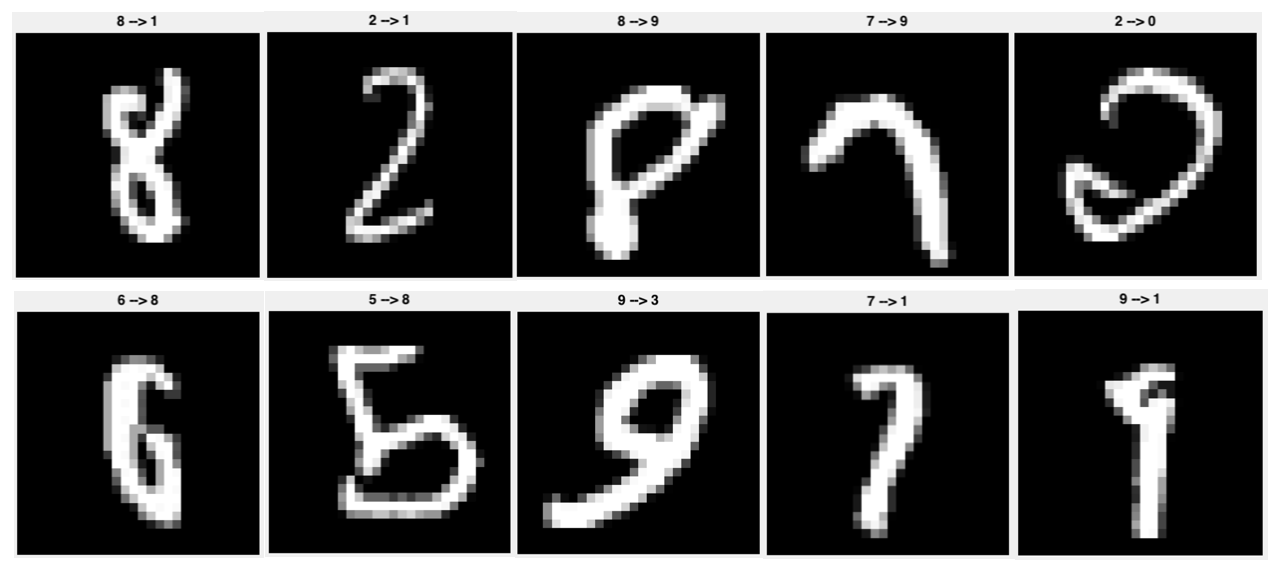
\includegraphics[scale=0.4]{gaussian_mis}
\caption{Examples of test images that are misclassified by the Gaussian model.}
\label{fig:gaussian_mis}
\end{figure}

Let us examine the Gaussian model more closely. Figure~\ref{fig:meangaussian} shows the mean vectors for each digit, namely, the estimated values of $\mu_j \in \R^{784}$, displayed as $28 \times 28$ images. Notice that the $\mu_j$ in Figure~\ref{fig:meangaussian} look identical to the mean vectors $p_{ji}$ from the Naive Bayes model in Figure~\ref{fig:meannaive}, because in both cases we obtain the mean vectors simply by averaging the training examples (except that in the Naive Bayes model we are averaging the binarized images).

\begin{figure}[h!]
\centering
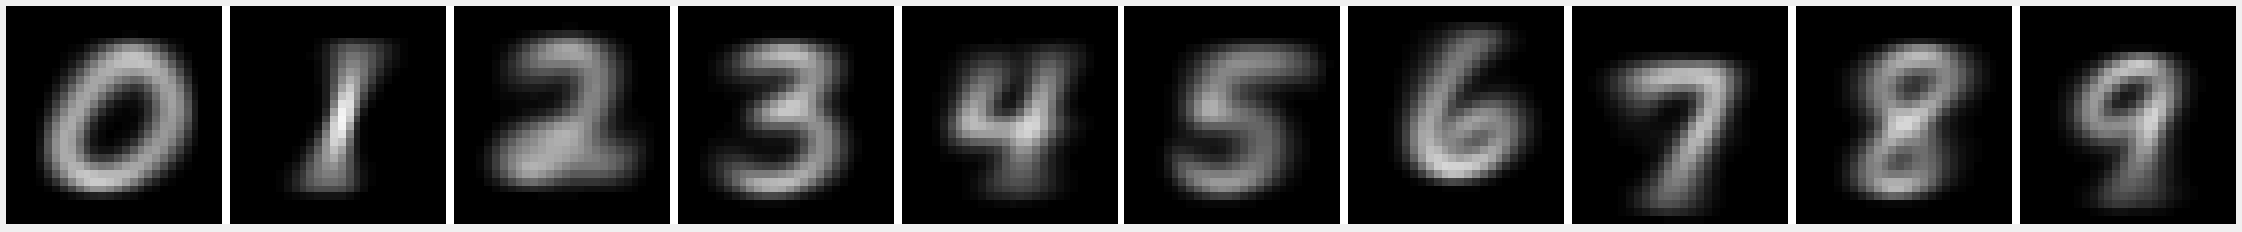
\includegraphics[scale=0.4]{meangaussian}
\caption{Mean vectors for each digit (the estimated $\mu_j$'s).}
\label{fig:meangaussian}
\end{figure}

In the Gaussian model we also have information about the correlations between pixel values, unlike in Naive Bayes where we assume all pixels are independent. Figure~\ref{fig:covgaussian} shows the estimated covariance matrix $\Sigma_j$ for digit $j = 0$ (left) and digit $j = 9$ (right). Both matrices look visually similar, with $\Sigma_0$ having stronger values on the corners than $\Sigma_9$. But it is difficult to understand what these covariance matrices mean, and whether they make sense for our problem. This is a general issue in complex problems: Once we are working with high-dimensional spaces, it can be hard to have a full understanding of what the model does, because our intuition does not guide us very well in high dimension.


\begin{figure}[h!]
\centering
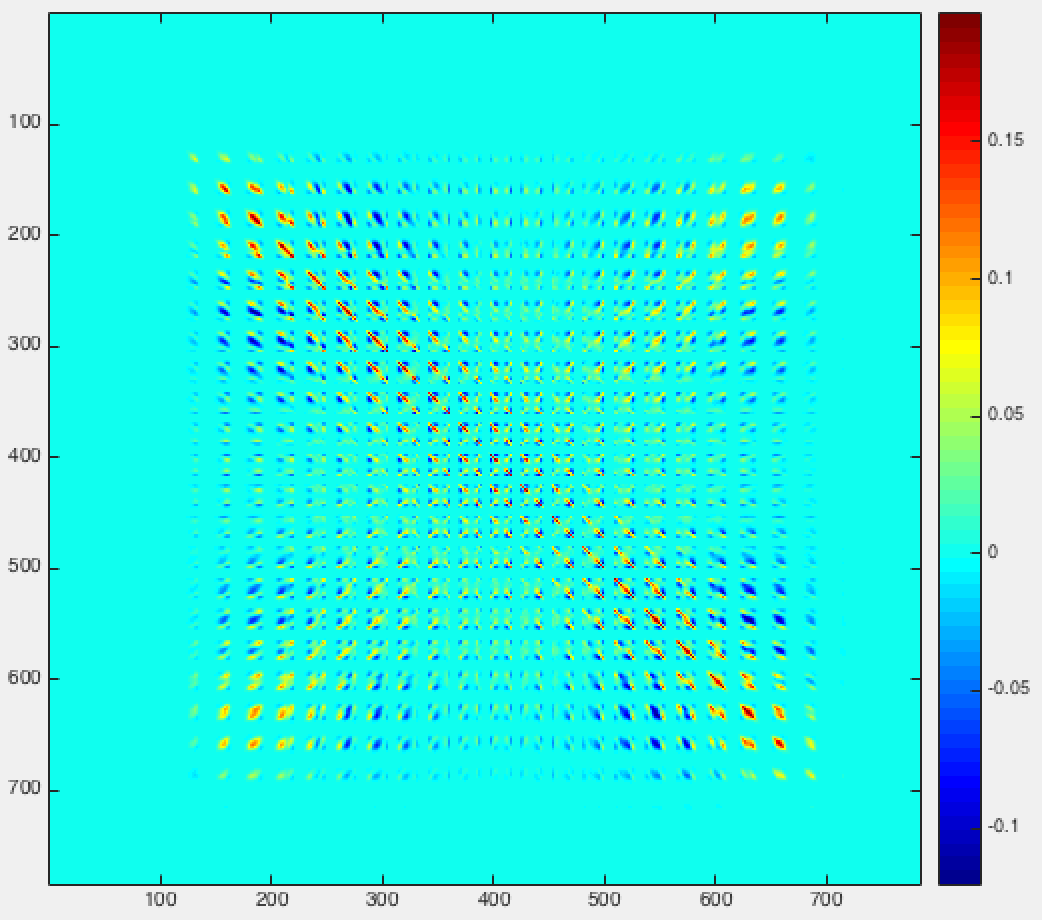
\includegraphics[scale=0.42]{cov0} ~~~~~~
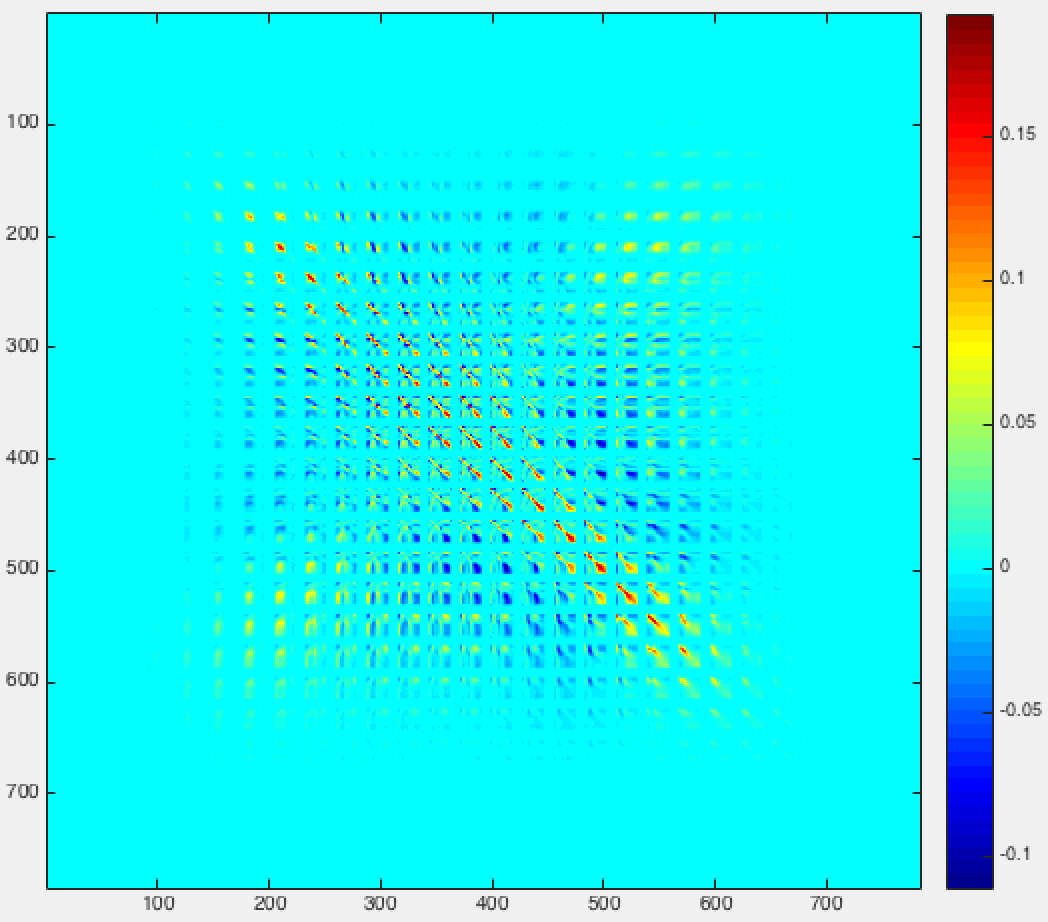
\includegraphics[scale=0.42]{cov9}
\caption{Estimated covariance matrix $\Sigma_j$ for digit $j = 0$ (left) and $j = 9$ (right)}
\label{fig:covgaussian}
\end{figure}


Finally, we can also generate samples from the Gaussian model we have trained, as shown in Figure~\ref{fig:gaussiansamples}. The first two rows are ordered based on the digits, while the last two rows are arranged in an arbitrary order. Can you still recognize the digits?

\begin{figure}[h!]
\centering
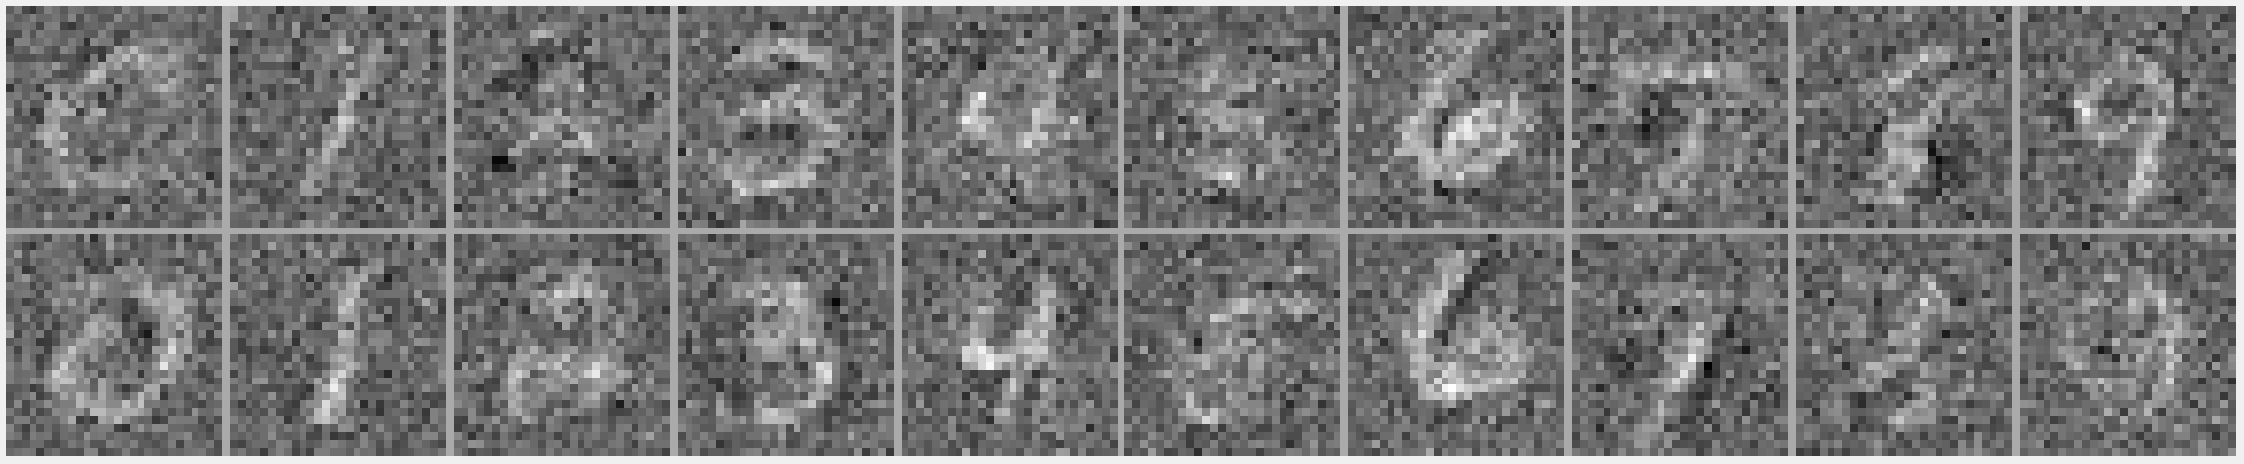
\includegraphics[scale=0.4]{gaussiansamples_ordered} \\
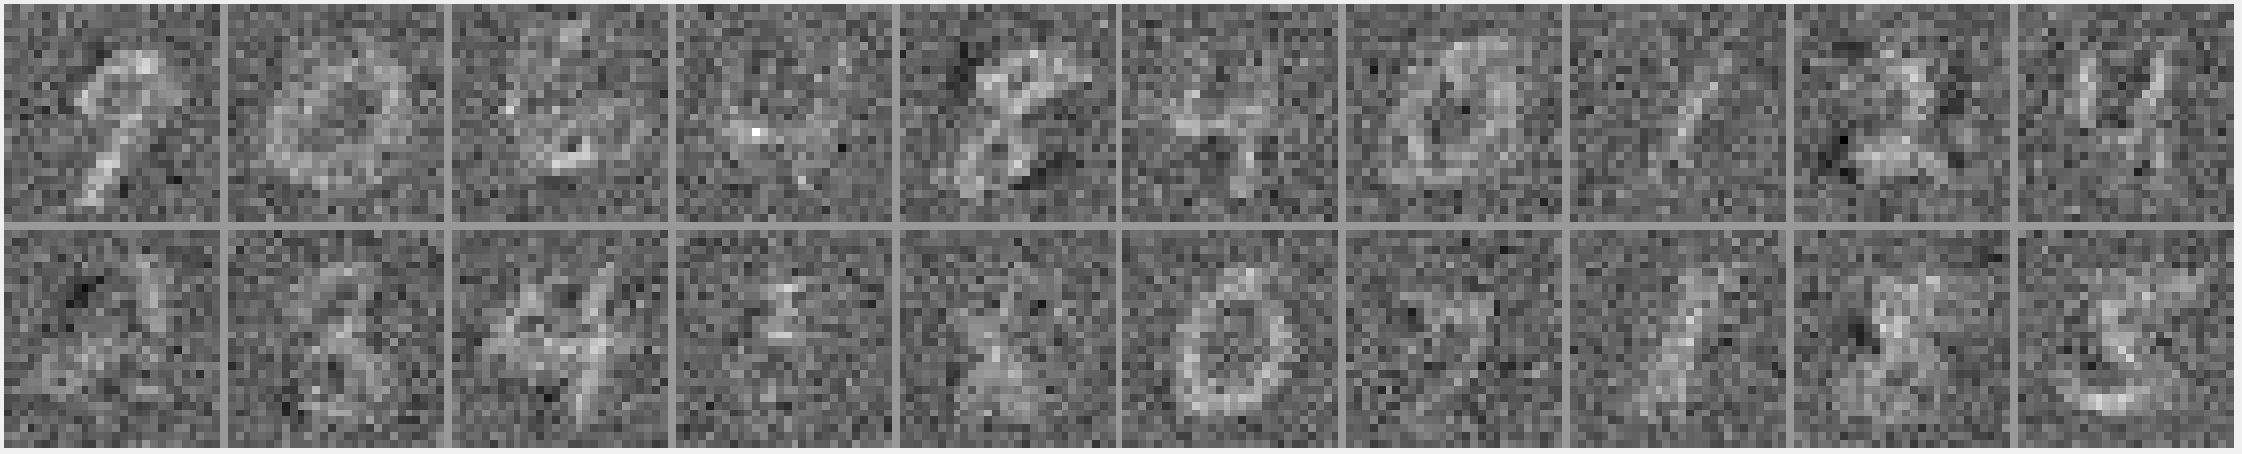
\includegraphics[scale=0.4]{gaussiansamples_random}
\caption{Some samples generated from the trained Gaussian model.}
\label{fig:gaussiansamples}
\end{figure}


We see above that the samples are very noisy and grainy, but we can still recognize the faint outline of the digits in the images. Note that since we are working with the Gaussian distribution over the entire real space $\R^{784}$, the pixel values in the generated samples can be negative, which does not make sense for real (grayscale) images. Yet we are still able to achieve a good performance in our digit classification task with this model. This again demonstrates that our model does not have to be very accurate, because the formalism of inference with Bayes' rule helps us do the rest of the work.




\end{document}

